\documentclass[tikz,border=5pt]{standalone}
\usepackage{fontspec}
\setmainfont{Times New Roman}
\usepackage{unicode-math}
\setmathfont{Cambria Math}
\usetikzlibrary{shapes.geometric,positioning,fit,backgrounds,arrows.meta,calc}

\begin{document}
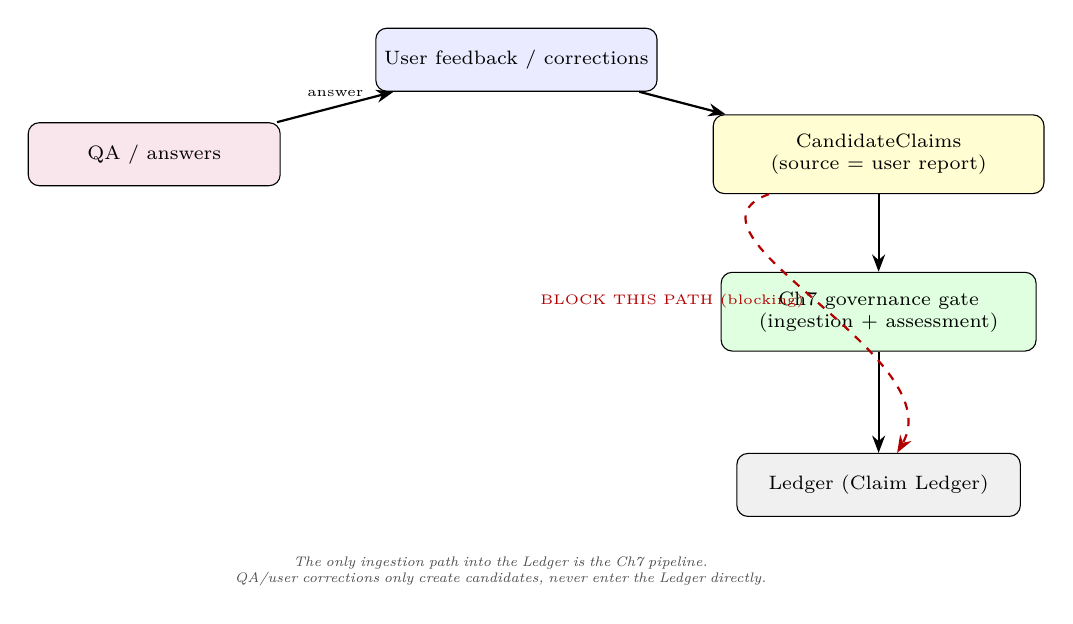
\begin{tikzpicture}[
  box/.style={rectangle, draw, rounded corners, align=center, font=\scriptsize, inner sep=3pt},
  arrow/.style={-{Stealth[length=2.2mm]}, thick},
  label/.style={font=\tiny\itshape, text=gray!60!black},
]

% === FEEDBACK LOOP WITH GOVERNANCE GATE ===
\node[box, fill=purple!10, minimum width=3.2cm, minimum height=0.8cm] (qa) at (-4.6, 3.0) {QA / answers};
\node[box, fill=blue!8, minimum width=3.2cm, minimum height=0.8cm] (fb) at (0, 4.2) {User feedback / corrections};
\node[box, fill=yellow!18, minimum width=4.2cm, minimum height=1.0cm] (cand) at (4.6, 3.0) {CandidateClaims\\(source = user report)};
\node[box, fill=green!12, minimum width=4.0cm, minimum height=1.0cm] (gate) at (4.6, 1.0) {Ch7 governance gate\\(ingestion + assessment)};
\node[box, fill=gray!12, minimum width=3.6cm, minimum height=0.8cm] (ledger) at (4.6, -1.2) {Ledger (Claim Ledger)};

\draw[arrow] (qa) -- node[above, font=\tiny] {answer} (fb);
\draw[arrow] (fb) -- (cand);
\draw[arrow] (cand) -- (gate);
\draw[arrow] (gate) -- (ledger);
\draw[arrow, red!70!black, dashed] (cand) to[out=200,in=60] node[left, font=\tiny, text=red!70!black] {BLOCK THIS PATH (blocking)} (ledger);

\node[label, align=center, text width=10cm] at (-0.2, -2.3)
  {The only ingestion path into the Ledger is the Ch7 pipeline.\\QA/user corrections only create candidates, never enter the Ledger directly.};
\end{tikzpicture}
\end{document}
